\documentclass[10pt]{article}
\usepackage{fullpage}
\usepackage{graphicx}
\usepackage{subfig} 
\usepackage{url}
\usepackage{amsmath}
\usepackage{multirow}
\usepackage[table,dvipsnames]{xcolor}
\usepackage[counterclockwise]{rotating}
%\usepackage{lscape}

\let\oldbibliography\thebibliography
\renewcommand{\thebibliography}[1]{%
  \oldbibliography{#1}%
  \setlength{\itemsep}{-2pt}%
}
\definecolor{sun4}{HTML}{CCCCFF}
\newcommand{\ccg}[1]{\cellcolor{sun4}{#1}}

\begin{document}

\title{Feasibility and Performance of PQC Algorithms on Micrtocontrollers %
\thanks{This work has been supported in part by NIST through
Grant no. 70NANB18H219}%
} 

\author{Brian Hession \and Jens-Peter Kaps}

\date{ECE Department, George Mason University, Fairfax, VA 22030, U.S.A.\\
%\email{\{bhession jkaps\\
\url{http://cryptography.gmu.edu}}%
%}

\maketitle

\begin{abstract}
The eXtended eXternal Benchmarking eXtension (XXBX), which was originally developed
to support the Competition for Authenticated Encryption: Security, Applicability, 
and Robustness (CAESAR), is a tool that can measure the performance of cryptographic 
algorithms on a variety of microcontrollers. We expanded XXBX from supporting 
hashing algorithms and authenticated ciphers to include benchmarking of key encapsulation 
methods and signature schemes in order to support the NIST Post-Quantum
Cryptography (PQC) standardization process. 
This paper describes the changes to XXBX which were necessary to support PQC and 
presents the first results we obtained for a variety of PQC candidates.
This is a work in progress and more PQC algorithms will be benchmarked as 
microcontroller friendly implementations are becoming available.
\end{abstract}

%\keywords{XXBX, ARM, IoT, Quantum, Cryptography}

\section{Introduction}

With quantum computers developing at an increasing rate, it is important to take into 
consideration the security implications that may come along with the technological progress. 
Quantum algorithms will make possible breaking many of the encryptions and algorithms used for 
key sharing in a reasonable amount of time~\cite{tobefound}.
%FIXME we need a better reference than Wikipedia. Didn't NSA make a statement?
An effort to preemptively design and implement 
quantum resistant security is vital to maintain proper security standards.

There are many algorithms and key sharing protocols proven to be quantum resistant that have 
already been developed. However, libraries that implement such algorithms focus on x86 
architecture and benchmarking. Embedded devices and the Internet of Things (IoT) lack extensive 
development. In 2018, IoT devices connected to the Internet numbered close to 23.14 billion. 
By 2025, that number is predicted to be closer to 75.44 billion~\cite{tobefound}.
%FIXME also here we need something more tangible as reference. 
Such a large subset of Internet 
connected devices cannot be left behind during the rise of quantum computing.

Two such libraries implementing quantum resistant cryptography are known as libpqcrypto~\cite{libpqcrypto} 
and the Open Quantum Safe Project (liboqs)~\cite{openquantumsave}. These libraries, however, target 
x86 and x86\_64 based architectures specifically. There are few efforts keeping IoT devices 
up-to-date~\cite{MALINA2018462}.

Embedded devices each come with their own strict memory and power constraints making the 
implementation of such instruction-heavy algorithms a very complicated effort. One such 
cryptographic library exists for ARM Cortex-M4 architectures known as pqm4~\cite{PQM4}. 
However, even this library overlooks some of the memory constraints of many devices. 
There exist tools to help the development, testing, and benchmarking on these specific 
environments—for example, eXtended eXternal Benchmarking eXtension (XXBX)~\cite{PK15,Kap16} which extends 
XBX~\cite{xbx} and SUPERCOP~\cite{SUP06}.  Since quantum computing is developing at an increased rate, 
it is vital for tools, such as XXBX, to keep up-to-date with the 
new emerging cryptographic standards.

\begin{figure}[ht]
    \centering
    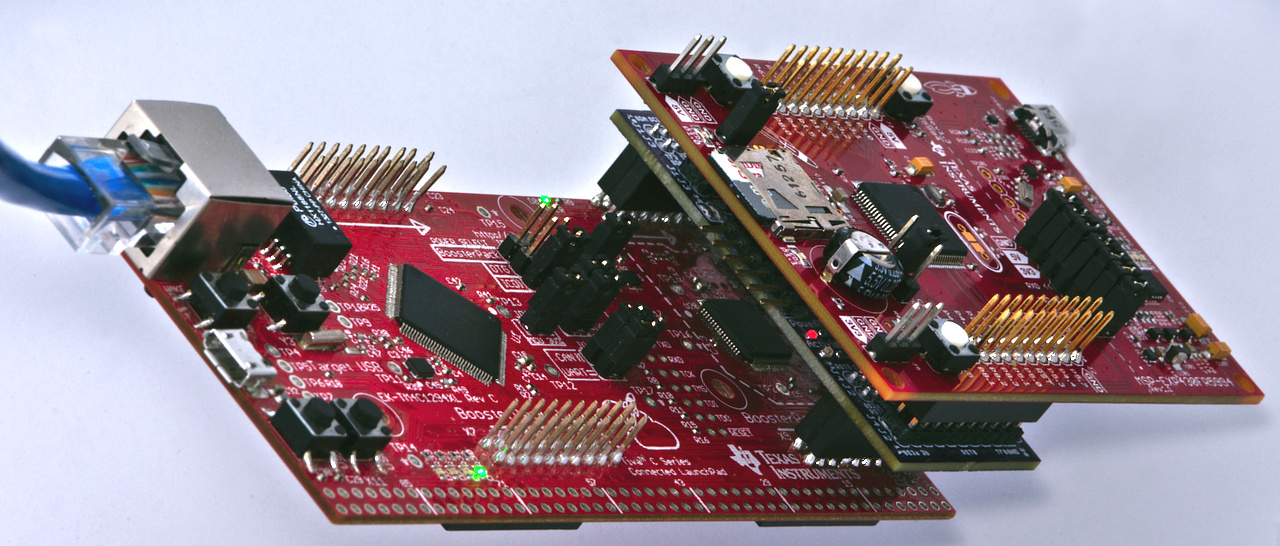
\includegraphics[scale=1.0]{../figures/xxbx-tilted}
    \caption{XXBX Setup}
    \label{fig:xxbx_setup}
\end{figure}

\section{Background (XXBX Design)}

XXBX can be broken into four parts: eXternal Benchmarking Software (XBS), eXternal 
Benchmarking Harness (XBH), eXternal Benchmarking Power (XBP), and 
eXternal Benchmarking Device (XBD). The XBS is the software used to interact with the XBH. 
The XBH acts as the control center and interface between the XBH and XBD. The XBP regulates 
the power and current going to the XBD. The XBD is the target device being benchmarked~\cite{xxbx}.

\begin{figure}[ht]
    \centering
    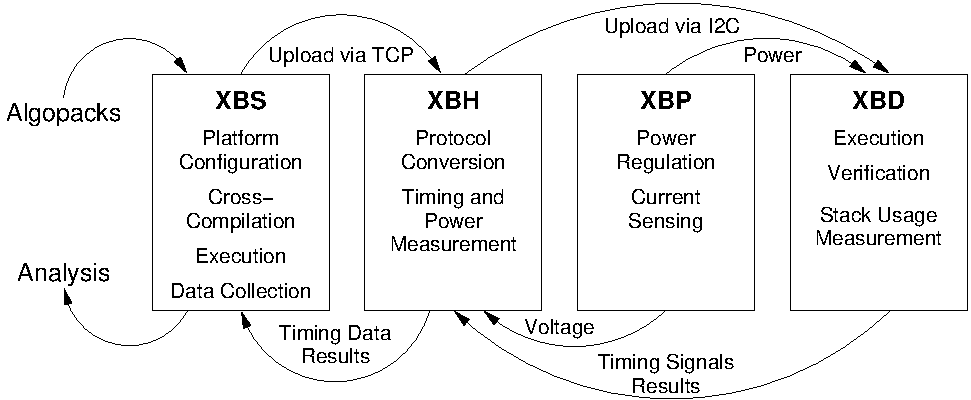
\includegraphics[scale=0.8]{../figures/xxbx_block.pdf}
    \caption{Block Diagram of XXBX Components}
    \label{fig:xxbx_block}
\end{figure}

\subsection{Flow}
The XBS will compile the benchmarking test cases and upload them via TCP to the XBH. 
The XBH will forward the test cases to the XBD via I2C and send a ``start execution'' signal. 
The XBD will execute the uploaded benchmarking test cases and return the results. 
Along with the results, the XBD will send back the clock cycles taken to execute the 
benchmark as well as the total stack usage.

During the execution, the XBH measures the power usage at regular intervals by taking 
samples from the XBP. After the execution is complete, the XBH will gather the power 
usage and results sent back from the XBD, package them, and send them back to the XBS 
for analysis [10].

The XBS will take these results and check for success. If successful, the results are 
uploaded to a database for further analysis. Figure~\ref{fig:xxbx_flow} depicts the flow of execution.

\begin{figure}[ht]
    \centering
    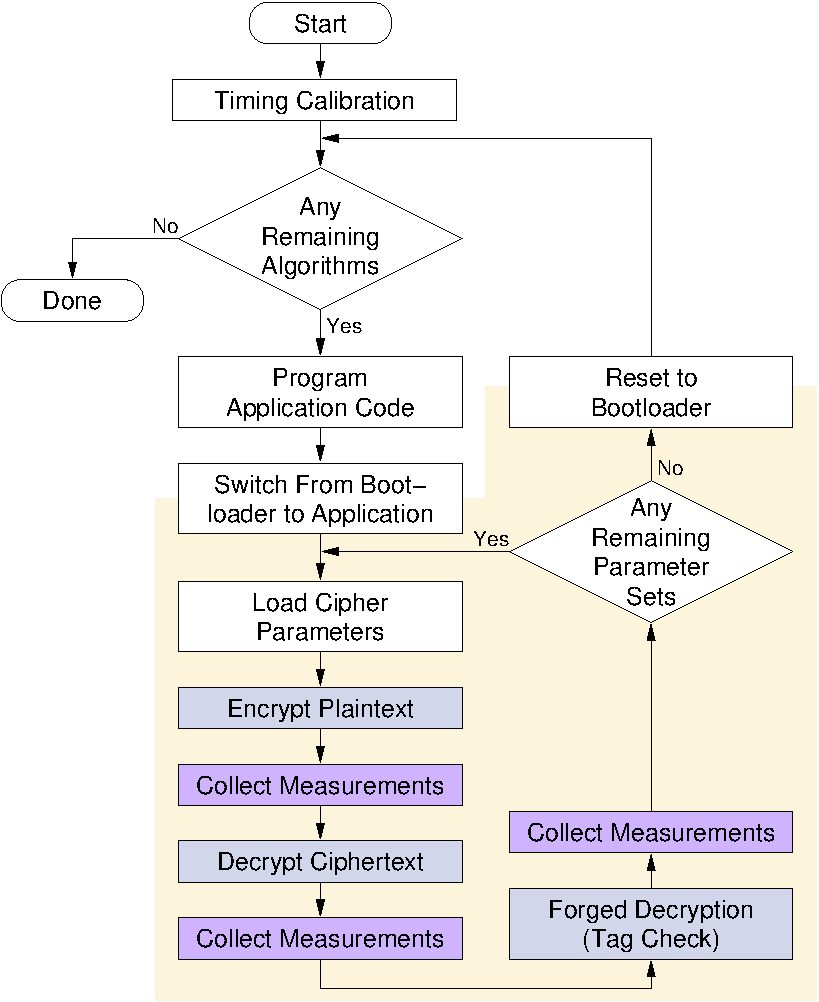
\includegraphics[scale=0.6]{../figures/xxbx_flow.pdf}
    \caption{XXBX Execution Flow}
    \label{fig:xxbx_flow}
\end{figure}


\subsection{XBD Bootloader}
The XBD needs to be loaded with a small bootloader that is able to receive commands 
and respond to the XBH. The main commands used for execution are the following:

\begin{enumerate}
  \item\emph{Program Flash Request}
     Loads the benchmarking test case application to the ROM.
  \item\emph{Timing Calibration Request}
     Calibrates the timing differences between the XBH and the XBD to allow for proper 
     timing measurements.
  \item\emph{Start Application Request}
     Switches the execution from the bootloader to the benchmarking test case application.
\end{enumerate}

\subsection{XBD Application}
The application can be considered an extension of the XBD bootloader code. These test 
cases are compiled with a specific cryptographic operation and algorithm. This creates 
portable code that sits within the ROM that the XBD switches to upon receiving the start 
application request.

A wrapper that the XBD bootloader understands connects the application and bootloader. 
To provide general support for all cryptographic operations, there only exists two buffers 
for execution of tests: parameter buffer and result buffer. The sizes of these buffers 
are decided at compilation and are unique to the cryptographic algorithm. It is up to the 
wrapper to compute the correct addresses of the parameters and results.

\subsection{XBS}
The XBS comprises of a collection of Python scripts. These scripts complete three main 
functions: compilation, execution, and data recording. 

A configuration file sets the cryptographic operation, the algorithm, the specific 
implementation to test, and the parameters needed to run the test. During compilation, 
the XBS will grab the specified implementation and the XBD wrapper code needed to execute 
the operation. Header files following the libcrypto format are generated and the code 
is compiled along with any dependencies that may be needed.
Upon a successful compilation, the database is initialized with the components needed 
to properly execute the tests. These components include the follow.

\begin{itemize}
  \item Operation
  \item Algorithm
  \item Implementation
  \item Parameters
  \item N columns of operation-specific details
\end{itemize}

During execution, the compiled application is loaded to the XBD for execution. 
A checksum is performed if the checksum file is present during compilation. The checksum 
test is essentially a test of sanity. It tests the algorithm for correctness and ensures 
it follows the expected behavior of the chosen cryptographic operation. Afterwards, the 
benchmarking is performed. The number of unique tests executed is equal to the number of 
parameter sets specified. The configuration can specify the number of trials to run per 
parameter set.

\subsection{XBH}
The XBH application controls the execution and behavior of the XBD. It receives commands 
from the XBS and translates and performs the specified actions on the XBD.

The device which the XBH code runs on must have a frequency equal to or greater than the 
device being benchmarked for correct results. Timing calibration is needed between the XBH 
and XBD to correctly estimate the number of clock cycles required to execute the cryptographic 
algorithm. When the start execution signal is received from the XBD, the XBH will start timing 
the execution and gather power usage statistics. This stops when the XBD sends the 
execution ended signal. At which point, the XBH will translate the time taken to clock cycles 
on the XBD. It then asks for the results and stack usage from the XBD.
This all gets packaged and returned to the XBS for analysis.

\section{KEMs and Signature Schemes}

For XXBX to be useful for benchmarking quantum-resistant cryptography, the functionality 
must be extended to include key encapsulation methods and signature schemes. This 
functionality is required in two separate parts of XXBX: XBS and XBD.

\subsection{XBS Extension}
XBS needs to understand the structure and tests needed to support the new functionality. 
As noted before, XBS will initialize the database with the components needed to properly 
execute the tests. During the execution stage, it will grab these components to forward 
to the XBH. A translation is needed here to package the data into something that XBD will 
understand. Also, upon return, the data will need to be translated back into something XBS 
can analyze. This translation should be dependent on the operation but general enough to 
support many different implementations.

Each trial for KEMs run each of the modes of operation in the following order: key generation, 
encapsulation, decapsulation, decapsulation failure. For signature schemes, the order is 
similar: key generation, signing, opening/verifying, forgery detection. The next mode of 
operation depends on the results of the previous mode. Therefore it is important each mode 
returns successfully or the trial is cut short, deemed a failure, and continues on to the 
next trial.

The parameters to package differ based on the mode of operation. And because there are 
different modes, and extra variable is needed to specify which mode the XBD will run.

The structure of execution results expected back in return follows a similar design. 
Because both KEMs and signature schemes depend on the result of the previous mode, these 
structures need to be kept track of during the life of the trial. Fig. 2 depicts both the 
structure of the parameters and the structure of the returned results.

For KEM key generation mode, no parameters are required—just the mode of operation while 
the results include both the public and secret key. For KEM encapsulation mode, the 
public key is written to the ROM at the next available block after the application binary. 
A pointer to this location is provided as a parameter while the results include the session 
key and ciphertext containing the session key. Lastly, for KEM decapsulation, the secret key 
is written to ROM (overwriting the public key) and a pointer to its location is provided as 
an argument along with the ciphertext containing the session key.

Signature schemes are similar. For key generation, no parameters are required and both the 
public and secret key are returned. For signing, the secret key is written to ROM and a 
pointer to its location along with the message are passed while the signature is returned. 
Lastly, for opening/verifying, the public key is written to ROM and a pointer to its location 
and signature are provided while the results include the verified message.

\begin{figure}[ht]
    \centering
    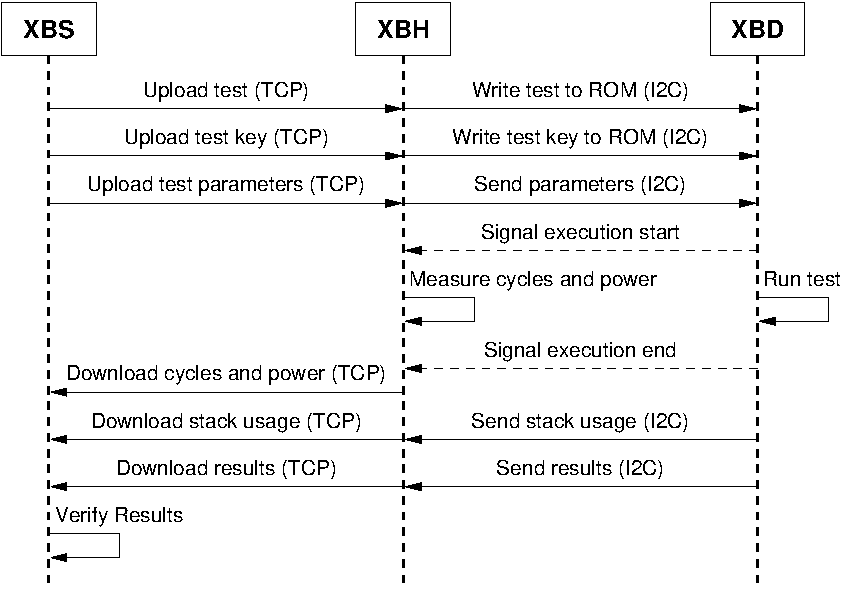
\includegraphics[scale=0.8]{../figures/xxbx_pk.pdf}
    \caption{XXBX Public Key Process}
    \label{fig:xxbx_pk}
\end{figure}

\subsection{XBD Extension}
XBD needs to translate the Start Application Request instruction to the intended operation. 
In order to do so, the data or parameters received by the XBS must match a format expected 
by the XBD. In turn, the results of the test must be packaged in a format the XBS is expecting.

Prior to unpacking the parameters, the XBD has no idea which mode is being performed. 
Because of which, the same buffer sizes are allocated regardless of the mode of operation. 
Therefore, the ROM usage calculated during execution do not accurately reflect the differences 
between modes and should be considered a general size for the algorithm. 
The size of the buffers are the largest required of the different modes of operation.

Regardless of success, the length of the returned results does not differ. 
This is particularly useful for ensuring incorrect decapsulation and detecting signature 
forgeries on the XBS side.

Unlike the XBS, each execution is independent of the previous.


\subsection{XBD Standalone}
An additional module was added to the XXBX structure. This XBD standalone mode creates 
an implementation of the algorithm in an environment without the XXBX overhead. It is a 
combination of XBD bootloader and XBD application stripped down to the core functions 
required to execute KEM and Signature operations.

This module automates the build process and allows for testing the algorithm in its purest 
form for accuracy instead of performance. It also allows for easy debugging with attached 
debuggers (such as GNU’s GDB).

Future work on this module will include an analysis of the stack during execution. 
In the typical XXBX environment, some of the stack is preserved for XBD application overhead. 
This module is designed to strip that overhead to its bare minimum and allow debuggers to 
test the logic of the implementation prior to running performance testing with XXBX. 
The automated build makes this process simple and extensible.


\section{IV. Quantum-Resistant Public Key Cryptography}

NIST released an initiative to design new quantum-resistant public key cryptographic 
standards. The algorithms analyzed are many of the candidates submitted to NIST for 
analysis [10].

SUPERCOP has a repository of KEM and Signature implementation that fix the XBX structure. 
This repository has many of the candidates for the new post-quantum standard. 
However, some of these algorithms are not capable of being built in embedded 
environments—particularly because of operating system calls.

Some additional implementations were pulled from pqm4 to replace those in SUPERCOP. 
Pqm4 has included some libraries and implementations of common dependencies required by 
a lot of these algorithms that work with the Cortex-M4 architecture~\cite{PQM4}. Pqm4 focused on 
Level III algorithms, so some work was required to fit Level I and Level V versions. 

\section{Target Device}

The ek-tm4c123gxl device was chosen to benchmark using XXBX. 
The ek-tm4c123gxl has been tested to work well with XXBX and has a large enough memory 
to work with a decent variety of algorithms. The device specifications are shown in Table I.

\section{Algorithm Candidates}

The candidates were split into their respective security levels defined by NIST. 
Table II defines the levels of classification.
For KEM algorithms, only levels I, III, and V apply. For signature schemes, all levels 
technically apply.

\subsection{XXBX Constraint}
The XBS network connection to the XBH will timeout during very long calculations on 
the XBD device. This will typically happen around 40 minutes or so.

\subsection{Target Device Signature Constraint}
The target device has available 32 kB of RAM. Most of the post-quantum signature 
algorithms exceed this constraint. Memory usage statistic from pqm4 are show below [6].
Most of the algorithms noted above exceed 32 kB worth of RAM. qTesla-I does work in the 
XBD-Standalone module but fails with the XBD application overhead.

\section{Results}

There are four categories of results: ROM usage, RAM usage, speed (in clock cycles), 
and energy consumption.

\section{Conclusion}

For embedded environments, the strict constraints due to limited memory size and power 
consumption makes developing IoT devices complicated. If execution time or power consumption 
are of greatest concern, both Kyber, New Hope, and Saber implementations are good candidates 
for KEM algorithms. However, if memory usage is of greatest concern, the Three Bears algorithm 
works better.

Sike takes an incredible amount of time to execute and is not a viable implementation for 
embedded environments.
XXBX is simple and adaptable. It will help users shift current cryptographic standards over 
to quantum-resistant public key cryptography in embedded environments.


\bibliographystyle{IEEEtran}
\bibliography{pqc-xxbx}


\end{document}

